\chapter{Discussion}
\label{ch-10}

\begin{refsection}[refs/ch-ten.bib]

This thesis was designed to explore how environmental impacts can be included in health technology assessment (HTA), with a focus on HTA for devices and drugs in the Australian reimbursement decision making context. It explored economic and environmental methods to estimate the environmental impact of healthcare technologies, reviewed methods to include these impacts in economic evaluations and HTA, and explored how these could form part of the Australian HTA decision making processes. This chapter outlines the principal findings of the research, summarises implications for research and policy, outlines the strengths and limitations of the body of work, and gives recommendations for future research. 

\section{Principal findings}
This thesis contains seven chapters that add new knowledge to the healthcare sustainability and health economics literature. Five of these have been published in peer-reviewed journals, and the remaining two have been submitted for publication and are currently under review. The findings of each chapter are summarised in Table 1. 

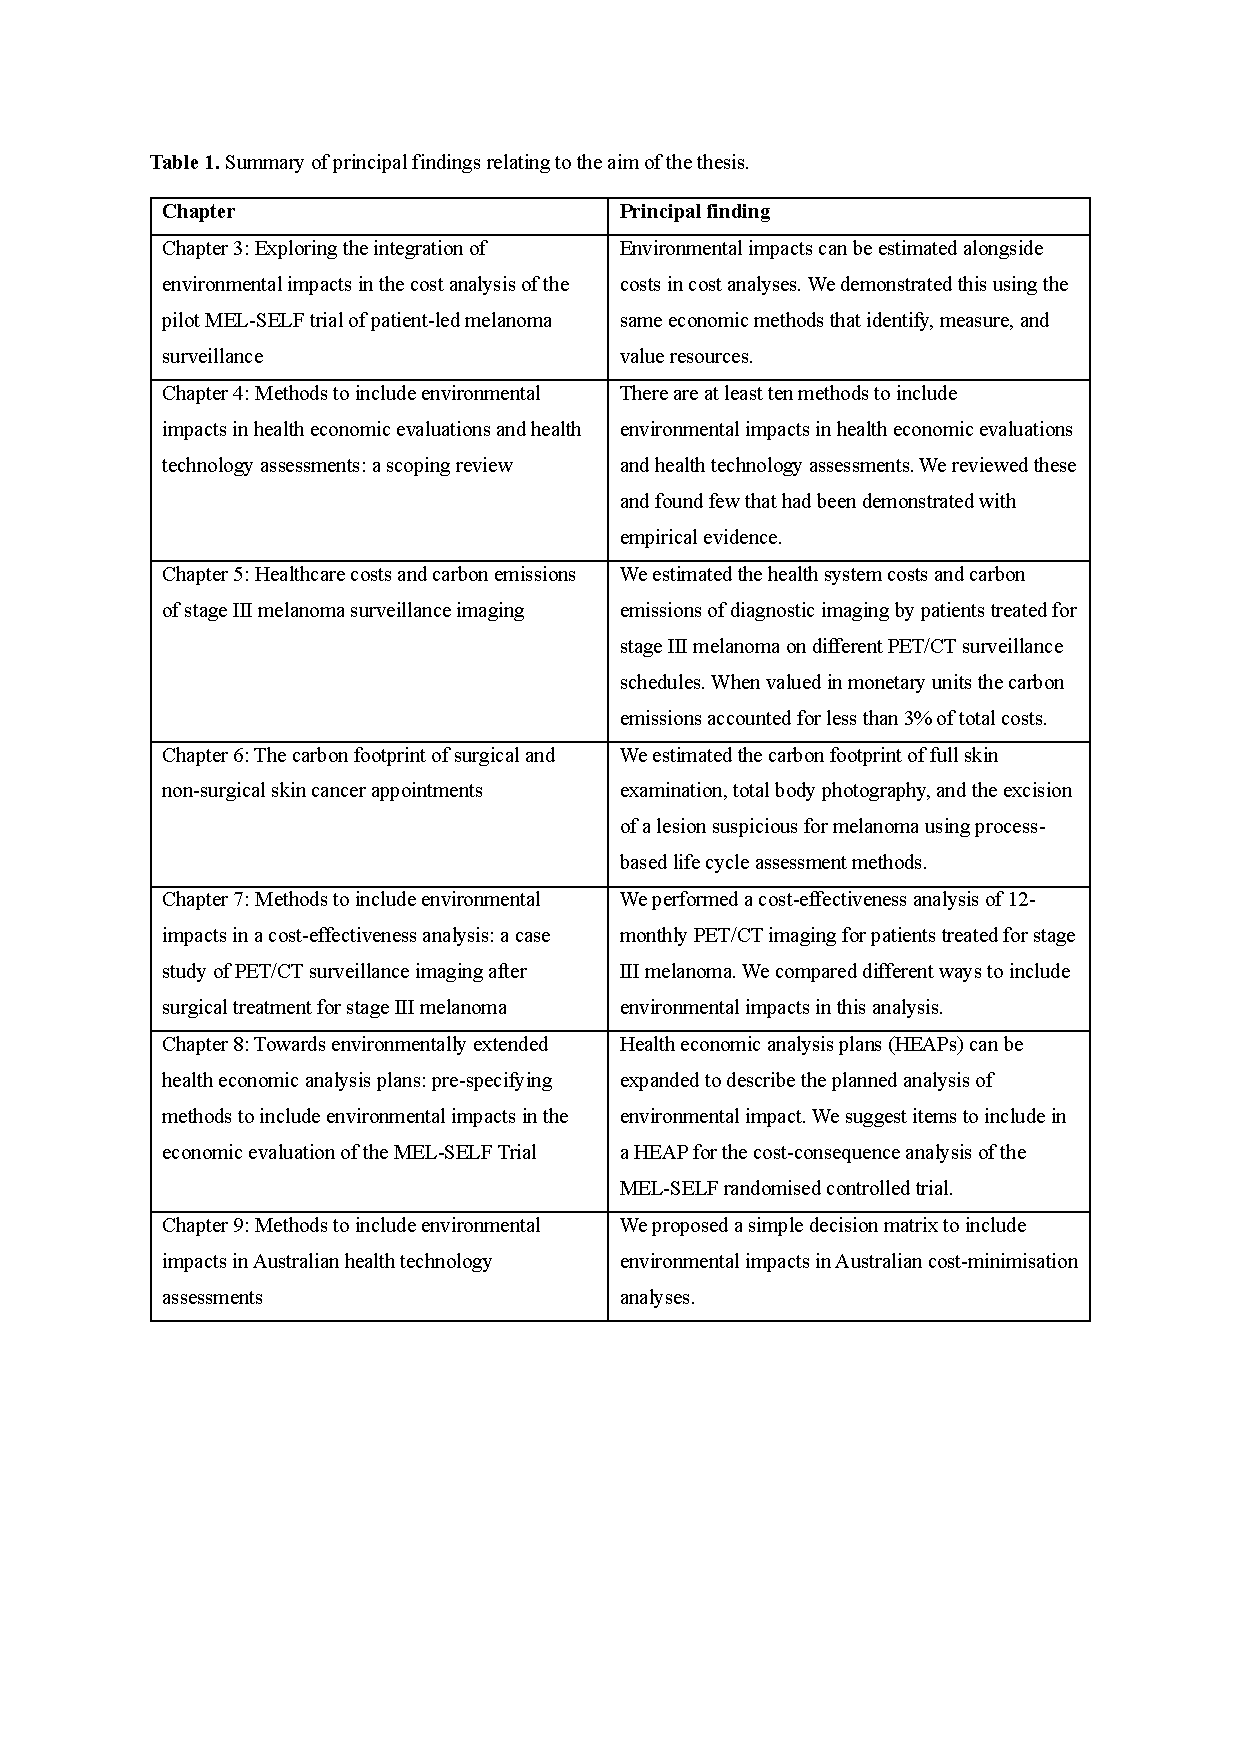
\includepdf[]{core-chapters/ch-10-tab.pdf}

Chapter 3 described an approach to include environmental impacts in a cost analysis and demonstrated this approach using the example of the MEL-SELF pilot randomised controlled trial. It was published in \textit{Applied Health Economics and Health Policy}. It found patients receiving patient-led and clinician-led surveillance, on average, cost the health system \$759 each, were associated with \$88 in productivity losses, incurred \$183 in out-of-pocket costs, and generated 10 kg CO$_{2}$-e from patient transport over the six-month study period. This study demonstrated environmental impacts, particularly carbon emissions, can be estimated alongside health costs in economic cost analyses, and doing so follows the same economic methods which identify, measure, and value healthcare resources. This study did not report any health outcomes, and it remained unclear how the environmental impacts could be included in full economic evaluations.

Chapter 4 reviewed and summarised evidence about methods to include environmental impacts in health economic evaluations and health technology assessments. It was published in \textit{Value in Health}. Two types of study were identified. The first identified, measured, and/or valued environmental impacts in a health economic context, with methods similar to those described in Chapter 3. The second demonstrated or described methods to include environmental impacts in an economic evaluation. Ten methods were grouped into four approaches: information conduit, parallel evaluation, integrated evaluation, and environment-focused evaluation. Only six studies demonstrated these methods, and none were from an Australian context. We found that while methods to include environmental impacts in HTA and economic evaluation existed, they had not been tested for use and further work was needed explore their application for real-world decision making. 

Chapter 5 estimated health system costs and carbon emissions of diagnostic imaging undertaken by patients on different PET/CT surveillance schedules for the follow up of stage III melanoma. It was published in \textit{Applied Health Economics and Health Policy}. It found patients in more frequent imaging schedules (i.e. scheduled imaging every 3-6 months) incurred higher healthcare costs and carbon emissions than patients managed with less frequent imaging schedules (i.e., scheduled imaging once per year). This study also explored the valuation of carbon emissions in monetary units and found emissions accounted for a small proportion (1.8-2.6\%) of total costs.

Chapter 6 estimated the carbon emissions of skin cancer clinic consultations. It is currently under review with \textit{Clinical and Experimental Dermatology}. The study used process-based life cycle assessment methods to estimate emissions in carbon dioxide equivalent units (CO$_{2}$-e). We explored three common reasons patients visit dermatology clinics for the diagnosis and treatment of skin cancer: full skin examination, total body photography, and the excision of a lesion. Carbon emissions were 11.11, 10.75, and 12.21 kg CO$_{2}$-e respectively. Patient transport was responsible for 10.72 kg CO$_{2}$-e.

Chapter 7 demonstrated methods to include carbon emissions in a cost-effectiveness analysis of different PET/CT surveillance imaging schedules for detecting distant metastasis after treatment for stage III melanoma. It was published in \textit{Value in Health}. The study used methods identified in Chapter 4, and inputs estimated in Chapters 5 and 6. Four methods were demonstrated: reporting emissions in parallel; the incremental carbon footprint cost ratio (ICFCR); the incremental carbon footprint effectiveness ratio (ICFER); and integrating emissions as a cost in the incremental cost-effectiveness ratio (ICER). The base case analysis (without environmental impacts) found 12-monthly PET/CT imaging was more expensive and more effective than no scheduled imaging, with an ICER of \$71,857 per false negative avoided. Carbon emissions were higher for 12-monthly imaging than no routine imaging. The ICFCR was 0.2 kg CO$_{2}$-e per additional dollar spent, and the ICFER was 17,331 kg CO$_{2}$-e per false negative avoided. When emissions were integrated as a cost the ICER increased modestly to \$74,017 per false negative avoided. In this example we found incorporating carbon emissions did not change the result of the CEA unless that valuation was relatively high, for example when the mortality accounting social cost of carbon (mSCC) was used. 

Chapter 8 described the health economic analysis plan (HEAP) for the MELanoma SELF surveillance randomised controlled trial and argued that guidelines for items to include in HEAPs should be expanded for studies including environmental impacts. It was published in \textit{Applied Health Economics and Health Policy}. 

Chapter 9 explored the application of methods to include environmental impacts in the Australian HTA decision making policy context. It is currently under review with the \textit{International Journal of Technology Assessment in Healthcare}. The article outlines the Australian policy context, evaluates potential methods, and proposes a simple decision matrix to include environmental impacts in a cost-minimisation assessment pathway.

\section{Implications}
The findings of this research have implications for health economists and for policy makers considering including environmental impacts in HTA and these are summarised in the following sections. 

\subsection{Implications for health economists and researchers}
There is a growing body of literature exploring how environmental impacts can be included in health economic evaluations and HTA, which was reviewed in Chapter 4 and by other recent studies.\cite{polisena_environmental_2018, pinho-gomes_incorporating_2022, guirado-fuentes_main_2023, desterbecq_inclusion_2023, antonazzo_health_2025} This work has largely focused on methodological descriptions and reviews, and, despite the empirical contributions of this thesis and of some other notable studies,\cite{de_preux_beyond_2018, kindred_exploratory_2024, dunbar_balancing_2025, marsh_incorporating_2016, kingma_exploring_2025} there is a lack of evidence demonstrating these methods. The cost-effectiveness analysis reported in Chapter 7 is the first Australian study of its kind and can be used by future studies seeking to include environment impacts in their analyses. There are two main implications of this research for health economists and other researchers.

First, economic methods are ideal for estimating the expected environmental impact of health technologies. In the empirical chapters of this thesis, we included carbon emissions in economic studies by identifying, measuring, and valuing resource use, such as healthcare services and patient travel. This is consistent with methods used in economic evaluations to estimate the costs and benefits of a technology.\cite{drummond_methods_2015} For example, in Chapter 5 we identified the use of diagnostic imaging tests, measured the number of times each test was used, and valued these using existing carbon emission estimates per test. Similar approaches were used in Chapters 3 and 7. This represents a modest addition to the work usually conducted in an economic evaluation to estimate the cost of the health technology, providing emissions factors for resources are already known.

Most economic evaluations do not usually derive resource unit costs de novo and instead rely on data from existing sources. The exception to this is in the case of micro-costing studies where there are no available estimates. Economic evaluations could follow the same principles for environmental impacts and rely on data from existing life cycle assessments (LCA), such as those indexed by the HealthcareLCA database or the recently announced Lancet MedZero.\cite{drew_healthcarelca_2025, watts_lancet_2025} Doing so would more efficiently use the limited healthcare-focused LCA workforce than conducting an LCA for every economic evaluation. It is also simpler for health economists to implement than requiring them to learn and conduct LCA within their studies. While there is currently a lack of high quality LCAs that can be relied on for economic evaluation inputs, LCAs only need to be conducted once per resource (for a particular time and place) and can then be relied on by future economic evaluations. 

If an LCA is conducted as part of the broader project it should be reported separately to the economic evaluation, as in the LCA reported in Chapter 6 for the cost-effectiveness analysis in Chapter 7. This ensures health economists can rely on their skills and do not need the specialist expertise or software required to conduct an LCA. It also ensures the LCA study is reviewed and published in sufficient detail and quality as to be useful to future economic evaluations. This might be less likely if the LCA is reported within an economic evaluation (i.e. with limited word count for the methods to facilitate replication).

Second, it showed including environmental impacts in economic evaluations is feasible and can be done in several ways. Once economic methods have been followed to estimate the environmental impact of the technology, it is methodologically simple to then include these in the evaluation, as described in Chapter 4 and demonstrated in Chapter 7. Different approaches and methods can be used by analysts with the most important differences being whether to integrate impacts into the evaluation (or consider them in parallel) and whether to value them in health, monetary, or environmental units. Consensus on the best approach has not been reached, especially in the context of health technology assessment, but this shouldn’t stop economic evaluations from exploring these methods further and contributing to much-needed empirical evidence of how proposed methods work in practice. Chapter 8 showed how to include environmental impacts in health economic analysis plans (HEAPs) for studies contributing to this body of work. This work might support, and be supported by, arguments for using a societal perspective, and for considering other broader costs and benefits in the economic evaluation.

In this thesis we found evaluations that include environmental impacts might reach the same conclusion about value for money as an identical evaluation that does not include environmental impacts. There are two reasons for this. First, in our case studies more costly health technologies had higher environmental impacts than less costly ones. While the cost of a technology and its carbon emissions are not directly linked, and carbon emission estimates based on monetary healthcare costs are unlikely to be valid,\cite{mcalister_how_2024} in the examples presented in Chapters 3, 5, and 7 we found that higher cost interventions also had higher emissions. Therefore, including emissions in the analysis may only reinforce the interpretation that would have been made without their inclusion. The exception to this may be when environmental impacts are integrated as a cost or benefit in a cost-effectiveness analysis. Here, considering the additional impacts may change the interpretation of value-for-money.

Second, and more importantly, the value of environmental impacts relative to the monetary cost of the technology or the health benefit appears to be small and difficult to interpret when common valuations are used. For example, in Chapter 7 of this thesis we found that when valued in Australian Dollars (AUD) and integrated into a cost-effectiveness analysis environmental impacts accounted for less than 3\% of total costs. This was true even when higher valuations (e.g. a higher social cost of carbon) were applied to the analyses and is consistent with the findings from other recent work.\cite{ducrot_integrating_2025} In Chapter 7 we identified the mortality accounting social cost of carbon (mSCC) as a potential value for carbon emissions. This is orders of magnitude higher than other social costs of carbon and did meaningfully impact the result of the cost-effectiveness analysis.

When environmental impacts are reported parallel to the economic evaluation the interpretation is difficult because we have little guidance about public and decision maker preferences for the trade-offs between health outcomes and environmental impacts. What would it mean for a technology that has an incremental cost-effectiveness ratio less than \$50,000 AUD but an increase of 100 t CO$_{2}$-e? Or, for a technology with an incremental carbon footprint effectiveness ratio of 100 t CO$_{2}$-e per quality adjusted life year gained? While these can be calculated and reported, their interpretation is difficult without understanding the preferences for the trade-offs taking place or the willingness-to-pay to reduce emissions. 

\subsection{Implications for policy makers}
As described in Chapter 1 and 9, Australian HTA does not require environmental impacts to be considered in by the applicants or the evaluators. The findings of this thesis show that health economic evaluations can be expanded to include environmental impacts, and there are plausible methods to include these in HTA for reimbursement decisions. However, further work is needed to address knowledge gaps before this can be done routinely.

Chapter 9 explores how guidelines for submissions to the Australian Medical Services Advisory Committee (MSAC) currently allow environmental impacts to be submitted as part of an application for reimbursement, and the HTA Review has proposed to explore how this can be done as part of an assessment of the technology’s cost-effectiveness. The primary challenge for the implementation of any of the feasible methods identified in this thesis is that we do not currently understand societal preferences for trade-offs between healthcare costs, health outcomes, and environmental impacts. Are we willing to spend more from the health budget to reduce carbon emissions and climate change? Would society trade potential health gains for individuals now, for carbon emissions reductions that benefit people in the future? What are society’s preferences for policy change related to the above to mitigate climate impacts? In Chapter 9 we proposed a simple decision matrix for Australia’s cost-minimisation pathway that partially avoids this issue by only considering environmental impacts when health outcomes are equivalent. While this may be useful in some scenarios, it is not known how often it would be useful. If HTA are to routinely consider environmental impacts, then this should be done systematically and not only in cost-minimisation analyses. 

There are also some practical implications for policy makers. First, guidelines for applications to MSAC, PBAC, and other similar bodies will need to be updated and made consistent to facilitate or require environmental impacts to be submitted with applications. This should contain specifics useful to the applicants, including what environmental impacts should be submitted, how they should be included, and how they will be considered. The answer to all these questions will depend on the context. It may also require additional expertise to be added to the advisory committees that review HTA applications and an upskilling of the epidemiological and health economic workforce to understand and report these data. Guidance will also need to be given about how this information will be interpreted once received by the committee. Considerations will need to be given as to how this might impact the speed of assessments and, at least initially, this is unlikely to be a compulsory requirement of HTA.

It remains unclear how often environmental impacts would influence HTA decisions. In their seminal textbook on methods for the economic evaluation of health care programmes, Drummond et al. suggest that the main “contribution of economic evaluation may not be in changing the decisions that are ultimately made but how they are made”.\cite{drummond_methods_2015} The findings of this thesis suggest that including environmental impacts may not change decisions that would have been made based on standard methods that do not include environmental impacts. However, as with the suggestion by Drummond et al. this does not mean it is not worthwhile. Rather, by including environmental impacts we can provide “proper accountability for the social choices made on behalf of others”.\cite{drummond_methods_2015} In the context of climate change this accountability is a worthwhile justification for including environmental impacts in economic evaluations. 

\section{Strengths and limitations}
The strengths of this thesis include its various methodological approaches, relying on costing, cost-effectiveness, and life cycle assessment methods to explore approaches to include environmental impacts in health technology assessment. It uses these alongside Australian case studies and policy perspectives to fill an important gap in the literature.

However, there are also limitations of this thesis. Limitations of each chapter are discussed in detail in the respective Discussion section of the chapter. Overall, this field has rapidly evolved since the first of the empirical chapters were designed and published. Because of this, methods and literature were less explored in those studies than in later Chapters. An example of this is the note in Chapter 4 that no study had explored the inclusion of environmental impacts on the benefits side of an economic evaluation as a QALY. However, by Chapter 7 a study was referenced demonstrating exactly that. Furthermore, we have not demonstrated all identified methods empirically and there remains a sizeable gap of evidence in this area. Future work should be coordinated and avoid further duplication of these research outputs.\cite{hensher_climate_2023}

\section{Future research directions}
Based on the findings of this thesis we make the following recommendations for future research directions.

First, we note in several chapters that the interpretation of environmental data is hindered by a lack of evidence about the preferences and attitudes of the public and of decision makers. HTA decisions are made on the behalf of society and reflect their preferences. Methods that include environmental impacts in HTA should be implemented based on an understanding of the preferences for these methods. Qualitative studies are needed to explore the methods discussed in this thesis, as well as public preferences for the potential underlying trade-offs between healthcare budgets, health outcomes, and environmental impact. Some pilot work has been conducted by NICE in the UK and future work is needed to explore these perspectives in contexts that consider including environmental impacts in their HTA processes, such as Australia.\cite{nice_nice_2023}

Second, there are outstanding economic methodological questions that need to be explored. While this thesis has focused on overall methods to include environmental impacts in HTA there are outstanding questions that need to be addressed for these methods to be routinely used. This includes questions about the time horizon of analyses, and how methods accounting for future damages are considered in evaluations of technologies with shorter time horizons; the discounting of environmental impacts and whether discounting future environmental impacts is appropriate or not; and the perspective from which the analysis is conducted (e.g., health system or societal). The health economic analysis plan presented in Chapter 8 suggests these be reported, but further work is needed to explore them empirically.

Finally, as prefaced in Chapter 8, we will include environmental impacts in the economic evaluation of the MEL-SELF randomised controlled trial. This will be informed directly by the findings of this thesis. Work is also needed to explore methods to include environmental impacts in economic evaluations conducted alongside randomised controlled trials that use other economic study designs, such as within-trial cost-utility analysis and Markov modelling. 

\section{Conclusion}
This thesis aimed to explore methods to include environmental impacts in health technology assessments. It described and evaluated several of these in the Australian healthcare reimbursement decision making context. It found economic evaluation frameworks are a useful way to estimate, present, and compare the environmental impact of health technologies. Further work is needed to understand how these can most usefully be implemented to inform HTA decisions in Australia and globally. 

\printbibliography[heading=subbibliography]
\end{refsection}